%!TEX root = practicum2.tex
We changed the stop condition, see \autoref{lst:b:stopCondition} and only checked for an intersection if $\dot{q} \times \dot{p} \neq 0$, see \autoref{lst:b:colinear}. Furthermore for some particular reason the algorithm consistently advanced the wrong edge after these additions, thus we swapped that around as well, see \autoref{lst:b:other}.\\

\lstinputlisting[float, firstline=194, lastline=200, label={lst:b:stopCondition}, caption={The new stop condition in  \t{algorithm_step_2()} in the class \t{convexPolygonIntersection}.}]{../convexPolygonIntersection.py}

\lstinputlisting[float, firstline=186, lastline=188, label={lst:b:colinear}, caption={The check on colinear line segments in \t{algorithm_step_2()} in the class \t{convexPolygonIntersection}.}]{../convexPolygonIntersection.py}

\lstinputlisting[float, firstline=207, lastline=216, label={lst:b:other}, caption={The swap in \t{algorithm_step_2()} in the class \t{convexPolygonIntersection}.}]{../convexPolygonIntersection.py}

The result of the extended \t{algorithm_step()} function on the provided degenerate example is presented in \autoref{fig:b:result}.

		\begin{figure}
			\centering
			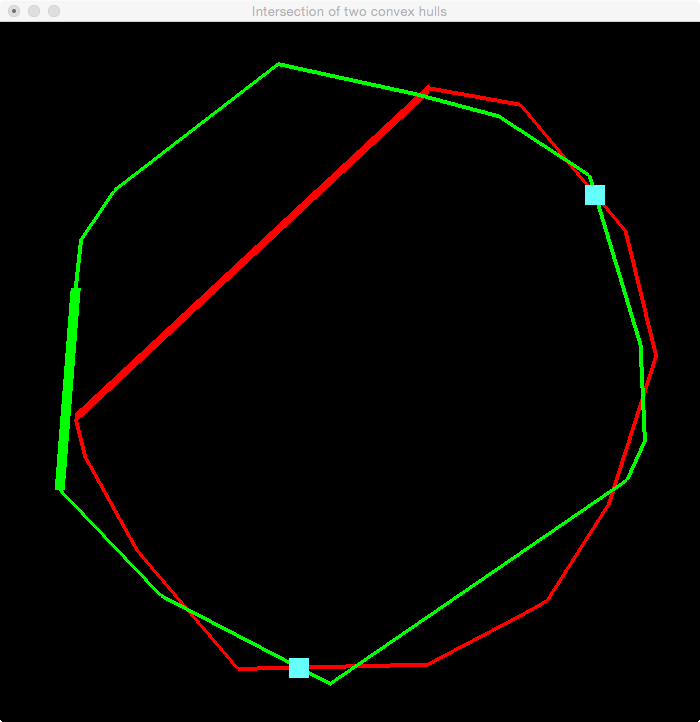
\includegraphics[width=0.4\textwidth]{./img/b_result}
			\caption{The final stage of the algorithm for the provided polygon \t{G} and \t{PDeg}. The found intersection points are shown in blue. The thicker edges denote the $\dot{p}$ and $\dot{q}$ at the last step.}
			\label{fig:b:result}
		\end{figure}	

\subsection*{Vertex on an Edge}
	This degeneracy causes the intersection of the vertex and the edge to be added twice to the list, since advancing one of the two edges does not remove the intersection, see \autoref{fig:b:vertexOnEdgeSteps}.

	This phenomenon is probably also the reason for the changed termination condition. 

	\autoref{fig:b:vertexOnEdge} shows the found intersections when polygon $P$ has one of its vertices on an edge of polygon $Q$.

		\begin{figure}
			\begin{subfigure}{0.24\textwidth}
				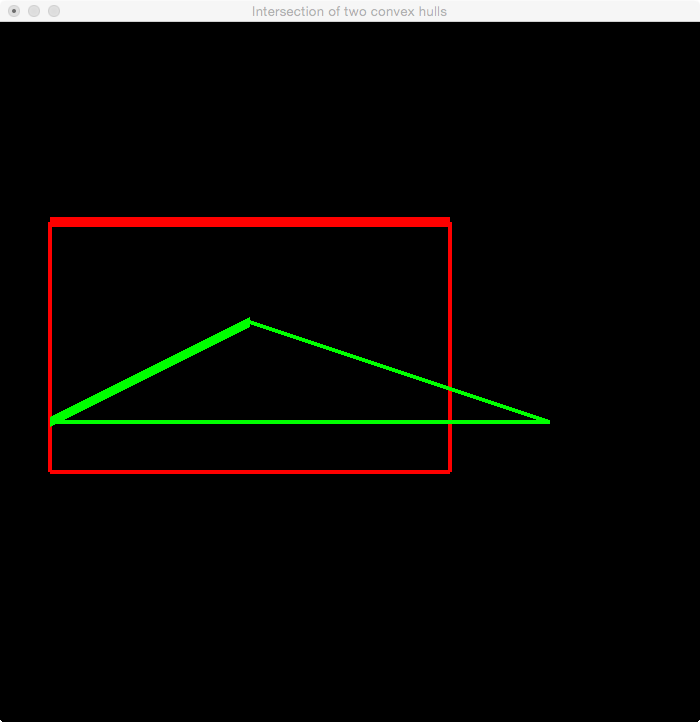
\includegraphics[width=\textwidth]{./img/b_step_0_deg_one}
				\caption{Step $i - 1$}
				\label{subfig:b:vertexOnEdge:step0}			
			\end{subfigure}		
			\begin{subfigure}{0.24\textwidth}
				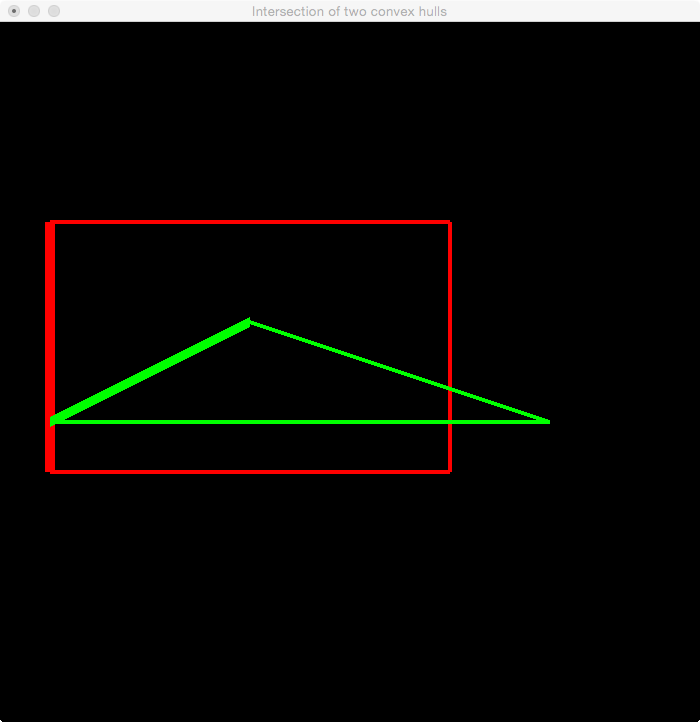
\includegraphics[width=\textwidth]{./img/b_step_1_deg_one}
				\caption{Step $i$}
				\label{subfig:b:vertexOnEdge:step1}			
			\end{subfigure}
			\begin{subfigure}{0.24\textwidth}
				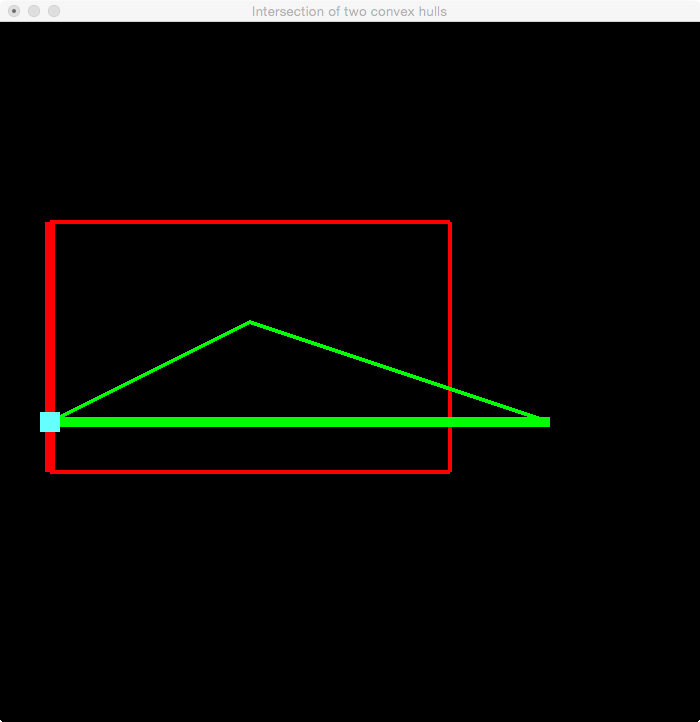
\includegraphics[width=\textwidth]{./img/b_step_2_deg_one}
				\caption{Step $i + 1$}
				\label{subfig:b:vertexOnEdge:step2}			
			\end{subfigure}		
			\begin{subfigure}{0.24\textwidth}
				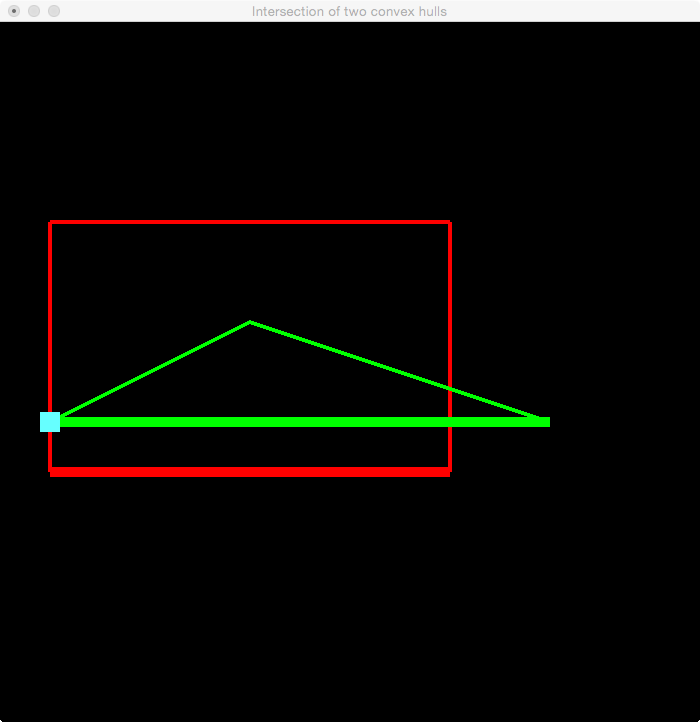
\includegraphics[width=\textwidth]{./img/b_step_3_deg_one}
				\caption{Step $i + 2$}
				\label{subfig:b:vertexOnEdge:step3}			
			\end{subfigure}				
			\caption{Four consecutive steps for the case where a vertex of polygon $P$ lies on an edge of polygon $Q$. Where step $i$ is the step where the intersection of the vertex on the edge is first found.}
			\label{fig:b:vertexOnEdgeSteps}
		\end{figure}

		\begin{figure}
			\centering
			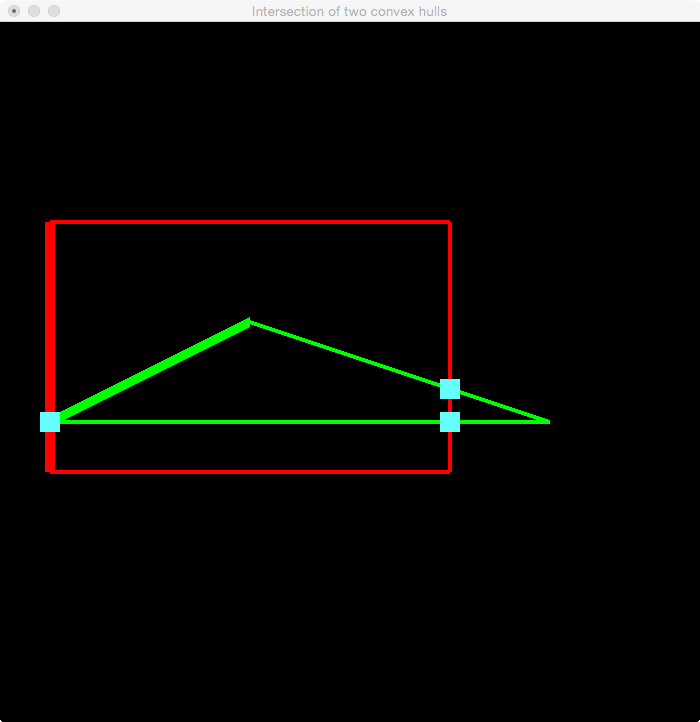
\includegraphics[width=0.4\textwidth]{./img/b_result_deg_one}
			\caption{The final stage of the algorithm for the case where one of the vertices of polygon $P$ lies on an edge of polygon $Q$. The found intersection points are shown in blue. The thicker edges denote the $\dot{p}$ and $\dot{q}$ at the last step.}
			\label{fig:b:vertexOnEdge}
		\end{figure}

\subsection*{Vertex on a Vertex}
	This degenerate case is still not handled well, since the intersection of the two overlapping vertices is found three times, see \autoref{fig:b:vertexOnVertexSteps}. The last time the intersection is found the algorithm terminates.

	However if we remove this condition the algorithm finds all intersections, see 

		\begin{figure}
			\begin{subfigure}{0.24\textwidth}
				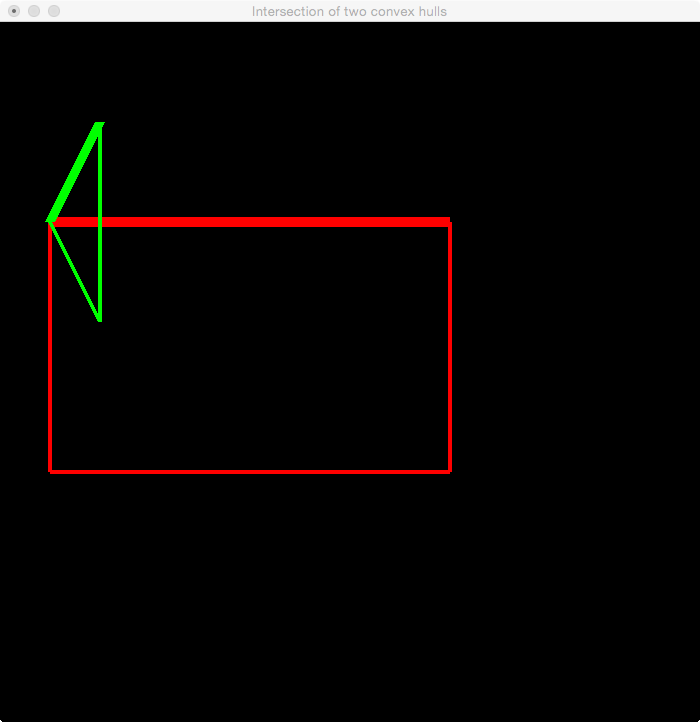
\includegraphics[width=\textwidth]{./img/b_step_0_deg_two}
				\caption{Step $i - 1$}
				\label{subfig:b:vertexOnVertex:step0}			
			\end{subfigure}		
			\begin{subfigure}{0.24\textwidth}
				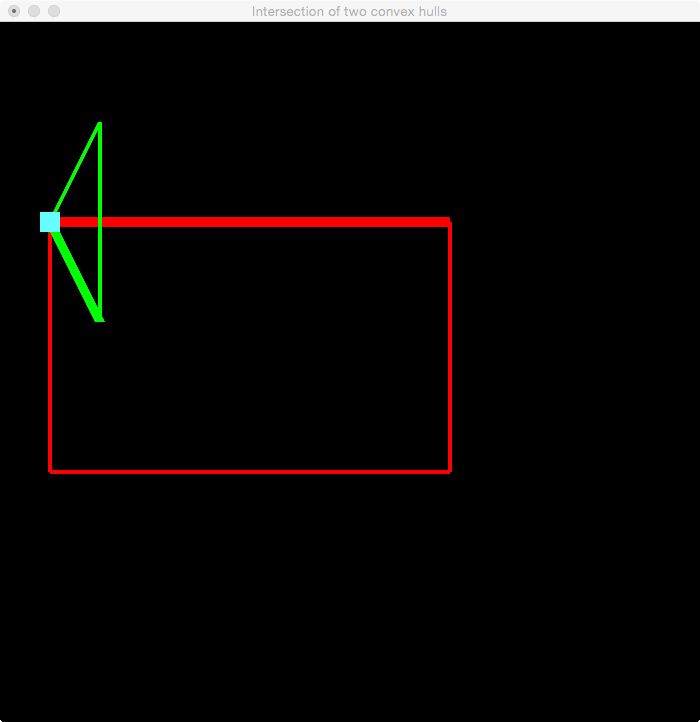
\includegraphics[width=\textwidth]{./img/b_step_1_deg_two}
				\caption{Step $i$}
				\label{subfig:b:vertexOnVertex:step1}			
			\end{subfigure}
			\begin{subfigure}{0.24\textwidth}
				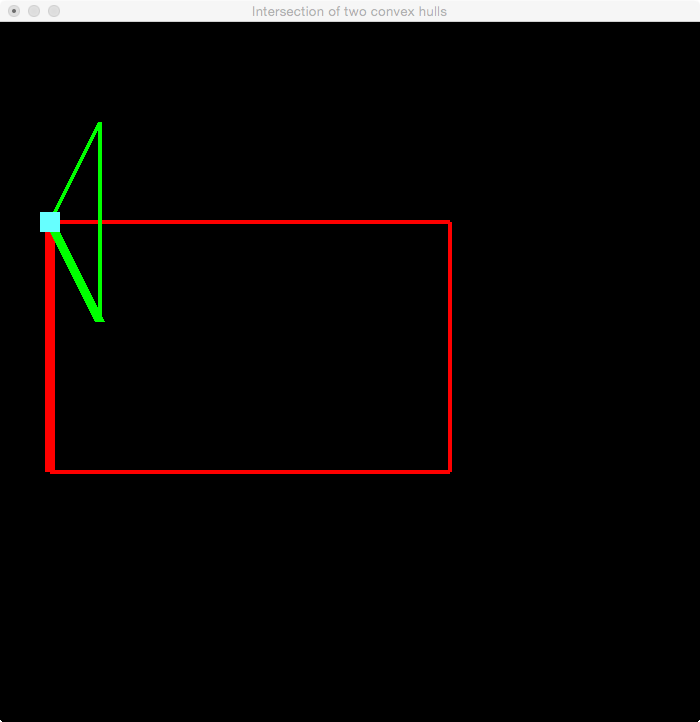
\includegraphics[width=\textwidth]{./img/b_step_2_deg_two}
				\caption{Step $i + 1$}
				\label{subfig:b:vertexOnVertex:step2}			
			\end{subfigure}		
			\begin{subfigure}{0.24\textwidth}
				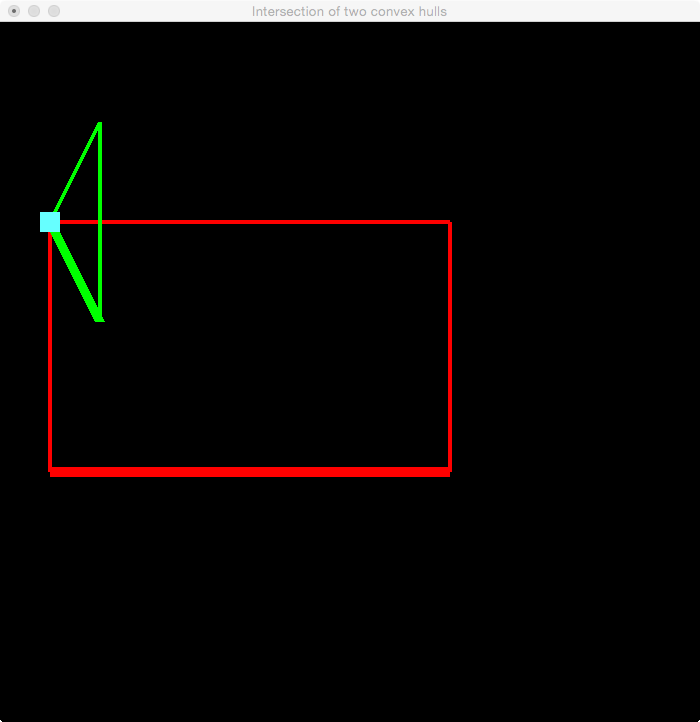
\includegraphics[width=\textwidth]{./img/b_step_3_deg_two}
				\caption{Step $i + 2$}
				\label{subfig:b:vertexOnVertex:step3}			
			\end{subfigure}				
			\caption{Four consecutive steps for the case where a vertex of polygon $P$ lies on an edge of polygon $Q$. Where step $i$ is the step where the intersection of the vertex on the edge is first found.}
			\label{fig:b:vertexOnVertexSteps}
		\end{figure}

		\begin{figure}
			\centering
			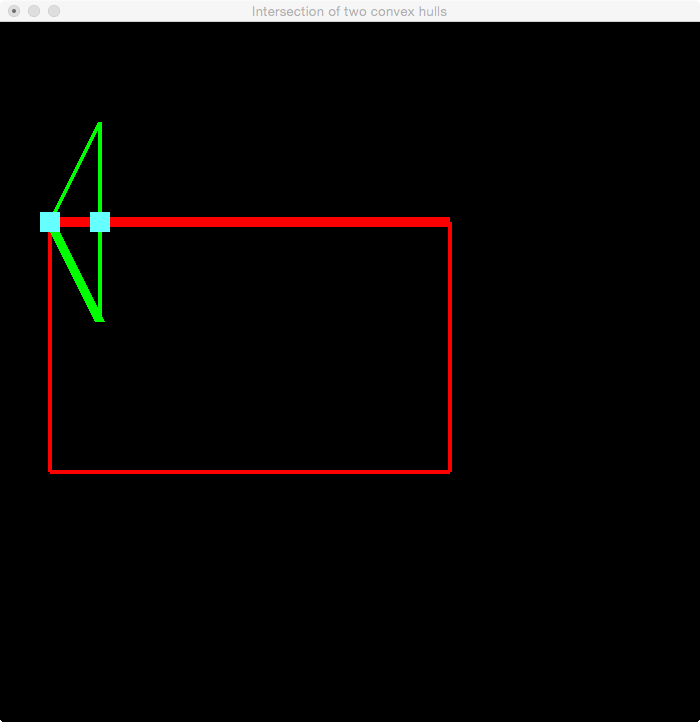
\includegraphics[width=0.4\textwidth]{./img/b_result_deg_two}
			\caption{The final stage of the algorithm for the case where one of the vertices of polygon $P$ lies on a vertex of polygon $Q$. The found intersection points are shown in blue. The thicker edges denote the $\dot{p}$ and $\dot{q}$ at the last step.}
			\label{fig:b:vertexOnVertex}
		\end{figure}

\subsection*{Edge on an Edge}
	For the results of the algorithm in the last degenerate case see \autoref{fig:b:edgeOnEdge}.

		\begin{figure}
			\centering
			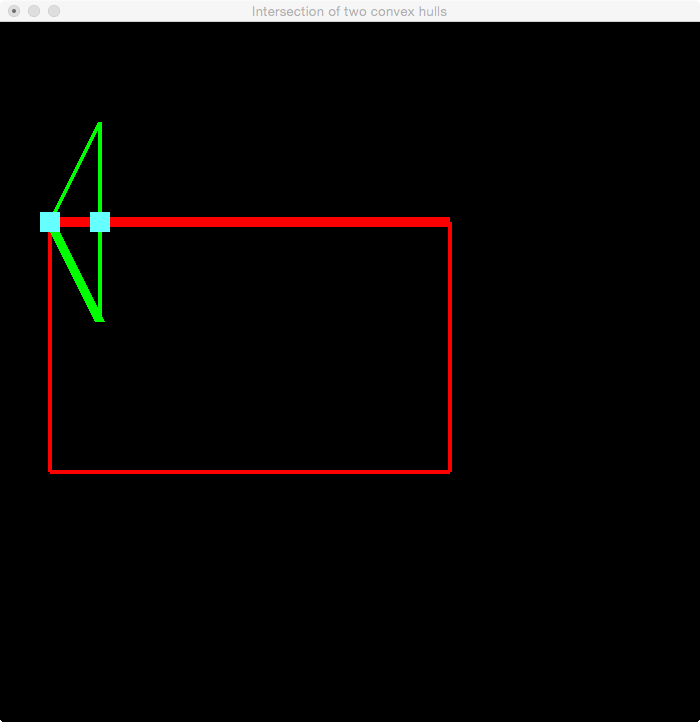
\includegraphics[width=0.4\textwidth]{./img/b_result_deg_two}
			\caption{The final stage of the algorithm for the case where one of the edges of polygon $P$ overlaps with and is colinear to an edge of polygon $Q$. The found intersection points are shown in blue. The thicker edges denote the $\dot{p}$ and $\dot{q}$ at the last step.}
			\label{fig:b:edgeOnEdge}
		\end{figure}